\documentclass[tikz,border=10pt]{standalone}
\usepackage{amsmath}
\usepackage{tikz}
\usetikzlibrary{shapes, arrows.meta, positioning, shadows}

\begin{document}

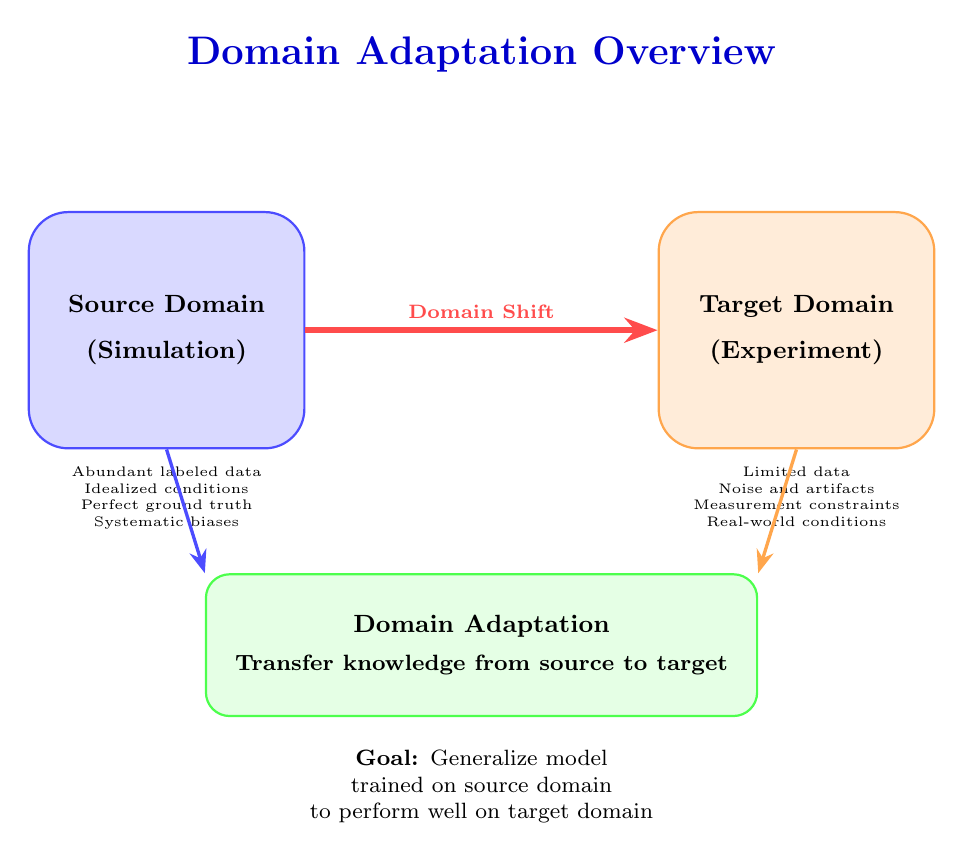
\begin{tikzpicture}[>=Stealth]

    % Title
    \node[font=\Large\bfseries, blue!80!black] at (0,0) {Domain Adaptation Overview};

    % Source Domain
    \node[rectangle, rounded corners=5mm, draw=blue!70, fill=blue!15, thick,
          minimum height=3cm, minimum width=3.5cm, align=center, font=\small\bfseries]
          (source) at (-4,-3.5) {
        Source Domain\\[0.2cm]
        (Simulation)
    };

    % Target Domain
    \node[rectangle, rounded corners=5mm, draw=orange!70, fill=orange!15, thick,
          minimum height=3cm, minimum width=3.5cm, align=center, font=\small\bfseries]
          (target) at (4,-3.5) {
        Target Domain\\[0.2cm]
        (Experiment)
    };

    % Domain Shift Arrow
    \draw[->, very thick, red!70, line width=2pt] (source.east) -- node[above, font=\scriptsize\bfseries, red!70, align=center] {Domain Shift} (target.west);

    % Characteristics - Source
    \node[below=0.1cm of source, font=\tiny, text width=3.2cm, align=center] {
        Abundant labeled data\\
        Idealized conditions\\
        Perfect ground truth\\
        Systematic biases
    };

    % Characteristics - Target
    \node[below=0.1cm of target, font=\tiny, text width=3.2cm, align=center] {
        Limited data\\
        Noise and artifacts\\
        Measurement constraints\\
        Real-world conditions
    };

    % Adaptation Strategy Box
    \node[rectangle, rounded corners=3mm, draw=green!70, fill=green!10, thick,
          minimum height=1.8cm, minimum width=7cm, align=center, font=\small\bfseries]
          (adapt) at (0,-7.5) {
        Domain Adaptation\\[0.1cm]
        \footnotesize Transfer knowledge from source to target
    };

    % Arrows to adaptation
    \draw[->, very thick, blue!70] (source.south) -- (adapt.north west);
    \draw[->, very thick, orange!70] (target.south) -- (adapt.north east);

    % Goal
    \node[below=0.3cm of adapt, font=\footnotesize, text width=6.5cm, align=center] {
        \textbf{Goal:} Generalize model trained on source domain\\
        to perform well on target domain
    };

\end{tikzpicture}

\end{document}
